\documentclass[a4paper]{article}

\usepackage{color}
\usepackage{url}
\usepackage[T2A]{fontenc} 
\usepackage[utf8]{inputenc}
\usepackage{graphicx}

\usepackage[english,serbian]{babel}

\newtheorem{primer}{Primer}[subsection]
\newtheorem{defn}[primer]{Definicija}


\usepackage[unicode]{hyperref}
\hypersetup{colorlinks,citecolor=green,filecolor=green,linkcolor=blue,urlcolor=blue}


\begin{document}

\begin{titlepage}

\newcommand{\HRule}{\rule{\linewidth}{0.4mm}}

\center 
	
\textsc{\LARGE Matematički fakultet}\\[3cm] 
	
\textsc{\Large Seminarski rad}\\[0.1cm]
	
\textsc{\large iz tehničkog i naučnog pisanja}\\[0.5cm] 
	
\HRule\\[0.4cm]
	
{\LARGE\bfseries Dajsonova Sfera}\\[0.2cm] 
	
\HRule\\[2cm]

\vspace{17\baselineskip}
		

	
	\begin{minipage}{0.4\textwidth}
		\begin{flushleft}
			\large
			\textit{Student}\\
			Dimitrije Vujko 196/2023
		\end{flushleft}
	\end{minipage}
\hspace*{1cm}
	\begin{minipage}{0.4\textwidth}
		\begin{flushright}
			\large
			\textit{Profesor}\\
			dr Jelena Graovac
		\end{flushright}
	\end{minipage}
	
	
\vfill\vfill\vfill\vfill 
	
{\large Beograd, \today} 
	
\vfill 
	
\end{titlepage}

\tableofcontents

\newpage

\abstract{
Konstrukcija svemirske megastrukture kao što je Dajsonova sfera predstavlja izuzetno kompleksan izazov. Tehnologija se stalno razvija kako bi odgovorila na rastuće energetske potrebe čovečanstva, koja se povećavaju usled napretka i sveprisutne potrošnje energije. Sa evolucijom društva i tehnologije, rastu i naše energetski zahtevi. Prema modelu Kardaševljeve skale, civilizacije se klasifikuju u tri tipa: tip 1, tip 2 i tip 3, svaki sa svojim specifičnim energetskim potrebama \cite{kskala}. Naučnici sprovode istraživanja kako bi bolje razumeli ove energetske dinamike. Dajsonova sfera se ističe kao potencijalno najveći i najčišći izvor energije koji možemo iskoristiti. Njen besprekoran dizajn čini je optimalnim rešenjem za zadovoljenje sveobuhvatnih energetskih potreba čovečanstva. 
}


\section{Uvod}
\label{sec:uvod}
Originalno predložena od strane legendarnog fizičara Fridmana 
Dajsona (eng.~{\em Freeman J. Dyson}), Dajsonova sfera ostaje jedna od najuzbudljivijih teorijskih ideja u svetu astrofizičara danas. Ideja je došla Dajsonu nakon čitanja romana {\em Star Maker} iz 1937. godine. U članku iz 1960. godine, Dajson je predložio članak u časopisu {\em Science} pod nazivom: {\em Potraga za veštačkim zvezdanim izvorima infracrvenog zračenja} \cite{firstpaper}.

Opisao je superstrukturu izgrađenu blizu ili
kod Sunca, koja bi mogla uhvatiti energiju Sunca i vratiti je na Zemlju. Čak i ako bi se to desilo, Sunce ne bi moralo snažno zavisiti od fosilnih goriva ili drugih postojećih izvora energije, čak i sa samo delom energije civilizacije.

Branitelji solarne energije znaju da samo mali deo ukupne energije Sunca pogađa Zemlju. Šta ako sakupimo svu solarnu energiju kao civilizacija? Tako da smo ponekad koristili vrstu Dajsonove sfere nazvane Dajsonova ljuska. Fizičar i astronom Freeman J. Dajson prvi put je otkrio ovu ideju kao misaoni eksperiment 1960. godine. Napredne civilizacije u našoj galaksiji neizbežno bi je koristile. Dajson tvrdi da potraga za dokazima postojanja takvih struktura može dovesti do otkrića naprednih civilizacija drugde u galaksiji.
U poslednjih nekoliko godina, astronomi su istraživali tu mogućnost sa čudnom zvezdom poznatom astronomima kao \textbf{KIC 8462852} – popularno nazvanom {\em Tabijeva zvezda} po njenoj otkrivačici Tabeti Bojajan (eng.~{\em Tabetha S. Boyajian}). O svetlu ove zvezde se prvobitno mislilo da ukazuje na moguću Dajsonovu sferu. Ta ideja je odbačena, ali 2018. godine pojavile su se druge mogućnosti, poput korišćenja misije {\em Gaia} za potragu Dajsonovih sfera.


\subsection{Fridman Dajson}
Rođen je u Engleskoj i radio je kao civilni naučnik u Kraljevskom vazduhoplovstvu tokom Drugog svetskog rata. Diplomirao je na Univerzitetu Kembridž (eng.~{\em Cambridge}) 1945. godine sa diplomom iz matematike. Nastavio je na Univerzitetu Kornel (eng.~{\em Cornell}) kao doktorski student 1947. godine i radio sa Hansom Beteom i Ričardom Fajnmanom. Njegov najkorisniji doprinos nauci bio je ujedinjenje tri verzije kvantne elektrodinamike. Univerzitet Kornel ga je imenovao za profesora, ne obazirući se na to što nema doktorat. Zatim je radio na nuklearnim reaktorima, fizici čvrstog stanja, feromagnetizmu, astrofizici i biologiji, tražeći probleme gde se elegantna matematika može korisno primeniti. 


\section{Kardaševa skala}

Skala koju je Nikolaj Kardašev (russ.~{\em Кардашев}) razvio 1964. godine kategorizuje nivo razvoja civilizacije prema količini proizvedene energije i načinu proizvodnje \cite{kskala}. Prema ovoj skali, nivo civilizacije u univerzumu je podeljen u tri tipa: 

\begin{itemize}
\item Tip 1
\item Tip 2
\item Tip 3
\end{itemize} 

\begin{defn}
     Civilizacija Tipa 1 je u mogućnosti da u potpunosti iskoristi svu
energiju svoje planete.
\end{defn}

\begin{defn}
    Civilizacija Tipa 2 je u mogućnosti da iskoristi svu energiju svoje najbliže zvezde.
\end{defn}

\begin{defn}
    Civilizacija Tipa 3 je u mogućnosti da iskoristi svu energiju svoje domaće galaksije.
\end{defn}

Ovi nivoi civilizacije razvijaju se proporcionalno korišćenju energije i energetskim potrebama (Tabela \ref{table:energetsa_potrosnja}).

U \textbf{Tipu 1} civilizacije, kojoj pripadamo, ali ne ispunjavamo uslove, moramo koristiti sve čiste izvore energije na planeti. Da bismo dostigli nivo civilizacije \textbf{Tipa 2}, moramo uspešno koristiti svu energiju neke zvezde. Za civilizaciju \textbf{Tipa 3}, morali bi da korsitimo svu energije naše galaksije. Međutim, trenutno obezbeđujemo više od polovine energije koja je potrebna našoj planeti iz fosilnih goriva. Nove prognoze predviđaju da će fosilna goriva biti iscrpljena do 2050. godine. Nakon iscrpljivanja fosilnih goriva, korišćenje čistih izvora energije će se povećati, ali ovi čisti izvori energije neće biti dovoljni zbog rezultata razvijajuće tehnologije.

Mnogi smatraju da, ukoliko čisti izvori energije nisu dovoljni, nedostatak možemo nadoknaditi upotrebom nuklearnih elektrana. Međutim, ove elektrane su vezane za iscrpljive resurse naše planete, poput uranijuma i torijuma. Ako dođe do iscrpljenja ovih elemenata u budućnosti, suočićemo se sa pitanjem energetskog opstanka.

Pored toga, imperativ je da vodimo računa da ne nanosimo štetu ekologiji Zemlje i dobrobiti ljudi dok proizvodimo energiju kako bismo dostigli nivo civilizacije \textbf{Tipa 1}. Očuvanje ekosistema Zemlje treba biti od ključnog značaja u našim naporima ka razvoju čiste i održive energije.


\subsection{Šta će se desiti nakon dostizanja civilizacije tipa 1?}
Nivo civilizacije \textbf{Tipa 2} je nivo gde resursi energije na planeti nisu dovoljni i sada radi drugog izvora energije potrebni su nam različiti tipovi resursa, a to su druge planete i zvezde u našoj okolini, Sunce i zvezde u centru sistema naše planete.

Djsonova sfera je struktura okružuje celu zvezdu i može iskoristiti svu energiju koju ona proizvodi. Civilizacije \textbf{Tipa 2} najverovatnije će pronaći načine da iskoriste svu energiju svojih zvezda uz pomoć Djsonove sfere (ili slične) tehnologije. To su civilizacije koje mogu prikupiti svu energiju kojom zrači njihova zvezda, na primer, civilizacija koja može izgraditi Djsonovu sferu, može prikupiti do $2 \cdot 10^{13}J$  energije svake sekunde (što je sva energija koju možemo dobiti od Sunca). Alternativno, fuzijska snaga zvezde može se koristiti kao reaktor velike skale kako bi zadovoljila potrebe ove civilizacije.

U civilizacijama \textbf{Tipa 3}, biološki značaj će biti isprepleten sa tehnologijom. U takvim civilizacijama može biti vrlo teško definisati značaj.

Koristeći svu energiju proizvedenu u galaksiji u kojoj postoje, ove civilizacije poseduju ogromnu količinu energije ($\approx 4 \cdot 10^{36} W$). One mogu kolonizovati galaksiju, izvlačiti energiju iz stotina miliona zvezda, lebdeti u međuzvezdanom prostoru i zauzeti beskrajne planete.

Za ljude, pristup takvoj vrsti znači stotine hiljada godina evolucije, kako bi se postigao evolucijski napredak, kako bi se zadovoljile biološke i mehaničke potrebe. Ljudi koji su čisto biološkog porekla verovatno će biti smatrani nesavršenim, inferiornim ili nefunkcionalnim od strane svojih kibernetičkih saputnika.

\renewcommand{\arraystretch}{1.5}
\begin{table}[]
    \centering
    \begin{tabular}{ |p{3cm}||p{3cm}|p{3cm}|  }
        \hline
        Tip 1& Tip 2 & Tip 3\\
        \hline
        $\approx 1 \cdot 10^{16} W$  & $\approx 4 \cdot 10^{26} W$ &$\approx 4 \cdot 10^{36} W$ \\
        \hline
    \end{tabular}
    \caption{Energetska potrošnja tipova civilizacija}
    \label{table:energetsa_potrosnja}
\end{table}



\section{Dajsonova sfera}
Dajsonova Sfera je hipotetička vanzemaljska megastruktura koja je predložena kao rešenje za pitanje "Šta ako vanzemaljske civilizacije ne žele da komuniciraju?". Dva radoznala profesora Kokconi i Morison, razmišljala su o ovom pitanju i došla do zaključka da treba tražiti radio signale u svemiru (eng. \emph{Morison and Cocconi}), što je na kraju dovelo do stvaranja pokreta potrage za vanzemaljskom inteligencijom kada je Frenk Drejk počeo svoje istraživanje u projektu nazvanom \emph{Projekat Ozma} \cite{firstpaper}.

Godine 1960. profesor Friman Dajson predložio je da je to zaista moguće, i ako bi takva civilizacija postojala, bila bi izuzetno sposobna u korišćenju i upravljanju energijom za rad, kao i za zadržavanje radio emisija u potpunoj izolaciji \cite{firstpaper}.

Dajson je tada predložio da se nekomunikativne civilizacije mogu možda detektovati izvora infracrvenog zračenja emitiranog iz gravitacionih bunara oko mase zvezde, ukoliko koriste dovoljno velik protok energije u poređenju s prirodnim izvorima infracrvenog zračenja na istom delu neba.

Prema Kardashevovoj skali, civilizacija koja može stvoriti Dajsonovu Sferu i iskoristiti svu energiju zvezde bila bi kategorizovana kao civilizacija \textbf{Tipa 2}.

Zbog ogromnog obima veličine žive zvezde i energetskog izlaza u različitim stanjima nuklearne fuzije, civilizacija koja je stvorila takvu megastrukturu da obuhvati celu zvezdu morala bi koristiti gust materijal koji je sposoban da se održi pod masivnom gravitacionom silom domaće zvezde. S obzirom na to da bi količina fotona koji udaraju unutrašnju površinu sfere takođe bila zadržana, gotovo sigurno bi bio potreban otvor za takve pritiske i energiju kako bi struktura održala svoju celovitost bez kolapsa \cite{dajsonstanf}.

Postoji i faktor volumetrijskog proširenja materijala korišćenog u konstrukciji sfere, formula: $\Delta V=\beta\Delta T$ objašnjava da će, prema koeficijentu linearnog proširenja materijala (umnoženom sa 3 za zapreminsko proširenje), u kombinaciji sa nultim zakonom termodinamike, doći do otpadne toplote koja napušta samu strukturu.

Dajson je kasnije došao do zaključka da bi oblik Dajsonove sfere najverovatnije bio skup određenih solarnih panela koje se nalaze u orbiti Sunca. Takva vrsta Dajsonove sfere je kasnije nazvan Dajsonov roj.



\subsection{Konstruckija Dajsonove sfere}
Dajsonova sfera se prvi put pojavljuje kao tema u serijama i filmovima, ali kasnije su naučnici shvatili da se na tome može raditi. Dr. Stjuart Amstrong (eng. \emph{Stuart Amstrong}) je predložio niz koraka koje bismo morali preduzeti da bi konstrukcija ovakve megastrukture bila uspešna. \textbf{Dajsovnov roj} ( Slika \ref{slika:dajsonov-roj}) predstavlja vrstu Dajsonove sfere koja se sastoji od solarnih kolektora (predstavljaju vrstu ogledala) koje reflektuju zrake Sunca na određeno mesto, gde se sunčevi zraci transformišu u upotrebivu energiju \cite{dsbuild}.

\begin{figure}[h!]
\begin{center}
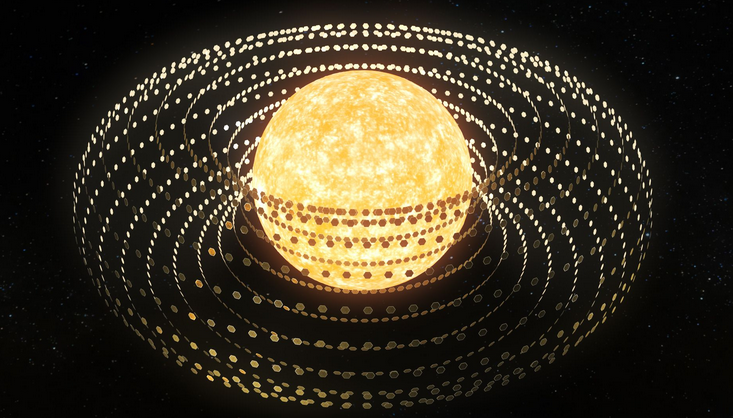
\includegraphics[scale=0.3]{Dajsonov-roj.png}
\end{center}
\caption{Dajsonov roj}
\label{slika:dajsonov-roj}
\end{figure}

Razbijen na pet osnovnih koraka, ciklus izgradnje izgleda ovako:

\begin{enumerate}
    \item Sakupljanje energije
    \item Rudarenje Merkura
    \item Pomeranje materijala u orbitu
    \item Izrada solarnih kolektora
    \item Ekstrakcija energije
\end{enumerate}

Navedni proces, koji je dr. Stjuart Amstrong opisao se odvija pod uslovom da imamo tehnologiju da kolonizujemo planetu Merkur, što će uostalom zapravo biti najveća prepreka izgradnje Dajsonove sfere.

Kako bismo mogli da iskoristimo 100\% energije Sunca, prvo moramo da prikupimo svu tu energiju korišćenjem \textbf{solarnih kolektora}. Za njihovu konstrukciju bi bilo potrobeno mnogo materijala, a sa obzirom da smo dostigli nivo civilizacije \textbf{Tipa 1}, nećemo imati ni blizu dovoljno materijala na našoj planeti. Zato planeta koja predstavlja najbolji izvor materijala i lokacije je u ovom slučaju Merkur.

Za prikupljanje većine energije koju proizvodi Sunce, potrebno nam je $3 \cdot 10^{16}$ \textbf{solarnih kolektora}, koje ćemo da lansiramo u orbitu Sunca. To je veliki broj i samim tim moramo da obezbedimo odredjenu količinu materijala, koje ćemo naći na Merkuru. 


Proces rudarenja i izrada solarnih kolektora predstavlja proces koji može da potraje, ali ako uzmemo u obzir da možemo da iskoristimo energiju koju solarni kolektor sakupi u svrhu izrade novih, tada proces veremenom postaje sve lakši i lakši. Od trenutka kada pošaljemo prvi solarni kolektor, do trenutka kada pošaljemo poslednji, biće potrebno od 10-15 godina, što predstavlja veoma malo vremena u poredjenju sa značajem izgradnje takve megastrukture. 



\subsection{Beli patuljci, život i Dajsonove sfere}
Zvezde se klasifikuju korišćenjem Hertzsprung-Russell (HR) dijagrama (Slika \ref{slika:hr_dijagram}), koji ih kategorizuje na osnovu sjaja i površinske temperature. Glavni tok čine zvezde koje fuzuju vodonik, zatim crveni divovi su evoluirane zvezde koje fuzuju više elemente, a beli patuljci su hladnije zvezde manje mase koje predstavljaju kraj evolucije.

Zvezde do otprilike 4 solarne mase ($4.989 \cdot 10^{33} grama $ )postaće beli patuljci, pod uslovom da ostane masa nakon izbacivanja materije tokom crvenog diva. Masa od 1,4 određuje da li će neobrtajuća zvezda postati beli patuljak \cite{whitedwarfs}.

Planetarni sistemi koji podržavaju inteligentni život očekuju da završe kao beli patuljci. Ako je međuzvezdano putovanje nepraktično, izgradnja Dajsonove sfere oko novog belog patuljka može održati civilizaciju. Faze crvenog diva, iako su dugotrajne, predstavljaju izazove za opstanak zbog promenljivih uslova.

Inteligentna civilizacija najverojatnije nastaje tokom glavnog života zvezde, preživljavajući fazu crvenog diva putem potencijalnog migriranja na dalju orbitu.


\begin{figure}[h!]
\begin{center}
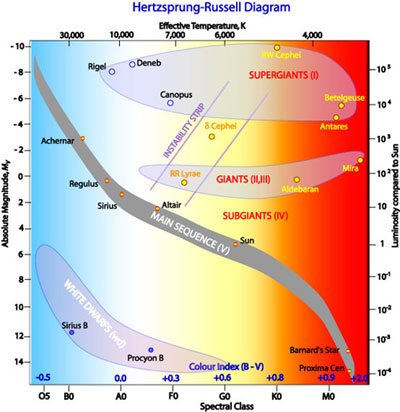
\includegraphics[scale=0.6]{HRdijagram.jpg}
\end{center}
\caption{Hertzsprung-Russell (HR) dijagram}
\label{slika:hr_dijagram}
\end{figure}


\section{Zaključak}
Izgradnja Dajsonove sfere predstavlja ambiciozan poduhvat koji, iako trenutno ostaje u domenu naučne fantastike, predstavlja tehnološki izazov s potencijalom za revolucionaran preokret u načinu života ljudi. Ovaj hipotetički projekat ne samo da bi omogućio visoko efikasno iskorišćavanje energije zvezde, već bi mogao označiti i prelazak na potpuno novi nivo energetske nezavisnosti i održivosti.

Uspostavljanje Dajsonove sfere bi zahtevalo pionirski rad u razvoju materijala, automatizaciji, svemirskim istraživanjima i inženjeringu. Ako bi ovaj poduhvat bio uspešno realizovan, mogao bi rezultirati revolucionarnim promenama u globalnom energetskom pejzažu, pružajući ogroman izvor čiste i neiscrpne energije.

Nadmašujući trenutne ekološke izazove i ograničenja fosilnih goriva, Dajsonova sfera bi mogla poslužiti kao ključna prekretnica ka održivijem i odgovornijem korišćenju resursa. Ovaj konceptualni projekat ne samo da bi obezbedio dovoljno energije za potrebe čovečanstva, već bi mogao označiti i prelazak ka budućnosti u kojoj je harmonija s prirodom centralna vrednost, postavljajući osnovu za prosperitet i dugoročno preživljavanje naše civilizacije.

\addcontentsline{toc}{section}{Literatura}
\appendix

\iffalse
\bibliography{seminarski} 
\bibliographystyle{plain}
\fi

\begin{thebibliography}{9}

\bibitem{firstpaper} F. J. Dyson, \emph{Search for Artificial Stellar Sources of Infrared Radiation} Science, 131, 1667-1668 (1960).

\bibitem{dsbuild} RealClear Science, \emph{How to Build a Dyson Swarm} by Ross Pomeroy, September 04, 2017.

\bibitem{whitedwarfs} Ibrahim Semiz and Salim Ogur, Bogazici University,
Department of Physics Bebek, \emph{Dyson Spheres around White Dwarfs}, Istanbul, March 2015.

\bibitem{dajsonstanf} Alastair Wee, \emph{The Dyson Sphere} Submitted as coursework for PH240, Stanford University, December 8. 2016.

\bibitem{kskala} Kardashev, N. S. \emph{Transmission of Information by Extraterrestrial Civilizations} Moscow, Russia, 1964.

\end{thebibliography}

\end{document}
